\documentclass[10pt,a4paper]{article}
\usepackage[utf8]{inputenc}
\usepackage{amsfonts}
\usepackage{graphicx}
\usepackage{indentfirst}
\usepackage{float}

\begin{document}

\title{Language Identification \\ with Contextual Translation}
\author{Alex Shah}
\date{12/4/17}

\maketitle

\section{Abstract}
   This project's goal is to combine different architectures of neural networks to form a functional translator with the ability to detect the input language and translate to the corresponding opposite language with contextual awareness. The resulting product combines a CNN classifier with tensor2tensor's transformer model for translation. Initially the languages chosen were English and Spanish but due to better availability of datasets in French, training was done with a French dataset. Any language with an appropriately processed dataset can be trained with.

\section{Introduction}
  Software translation is a massively useful tool to bridge the gap between cultures. Providing a software implementation for translation does not require the entire computation to occur on the device, but rather through training ahead of time. In this way, your cell phone does not need a desktop PC's compute power to leverage neural networks and the advances such technologies have made in machine translation. However, training the network, and the preparation for making a translator, does require a large amount of compute power and time.

  In order to minimize the amount of time required, we can make training more efficient by training both translation directions simultaneously. By using encoder/decoder as a basis for our model, languages and context are broken down into mathematical representations that the network uses to translate any language to any other. We do not need to train translation from language A to language B and vice versa, but can learn each language independently.

  By utilizing language agnostic training, we can improve the speed at which we train. We can train any language in the same time, without needing to retrain or cross train various languages when a need language is added. This concept applies to both the classifier and for translation. 

\section{Background}

\subsection{Language Classification}

  Classifying a given input is handled by a Convolutional Neural Network (CNN). It is crucial to quickly determine the input language as identifying the language is an intermediary step before translation. However, incorrectly determining the input language will create incorrect translations. Therefore it is important that the classification network is able to quickly but accurately detect the input language. A CNN is accurate with very few epochs of training. In as little as 10 epochs the accuracy is over 90\% for inputs of 70 characters.  

\subsection{Contextually Aware Translation}

  Strides have been made using deep learning and deep network models for Machine Translation (MT) accuracy, making MT ever more accurate in contextually aware translation. Sequence to Sequence networks (Seq2Seq) are built like an encoder/decoder. The encoded input text is examined to determine the decoded output in the target language. An attention mechanism is used to share information from previous input steps to help better inform output decoding. This is more efficient than bidirectionally sharing input and output values, but is also more accurate than less computationally intensive methods such as reversing input strings. Specifically, attention shares memory between the encoder steps and decoder to produce more contextually aware output. The encoder mechanisms in NMT models are used to build a thought vector from a given input. This vector captures context which is then decoded into the target language translation. The attention mechanism determines how much context is too little or too much, which enables the translation to capture and translate advanced syntactical structures such as gender agreement and other "long range dependencies" without overfit or poor context capture.

  Neural Machine Translation (NMT) advances with Google's tensor2tensor library, a specifically derived set of Seq2Seq and RNN based models focusing on accuracy and efficiency of training translation models. Models like Transformer have achieved some of the best accuracies in NMT. 
  
\clearpage

\begin{figure}[H]
  \begin{center}
    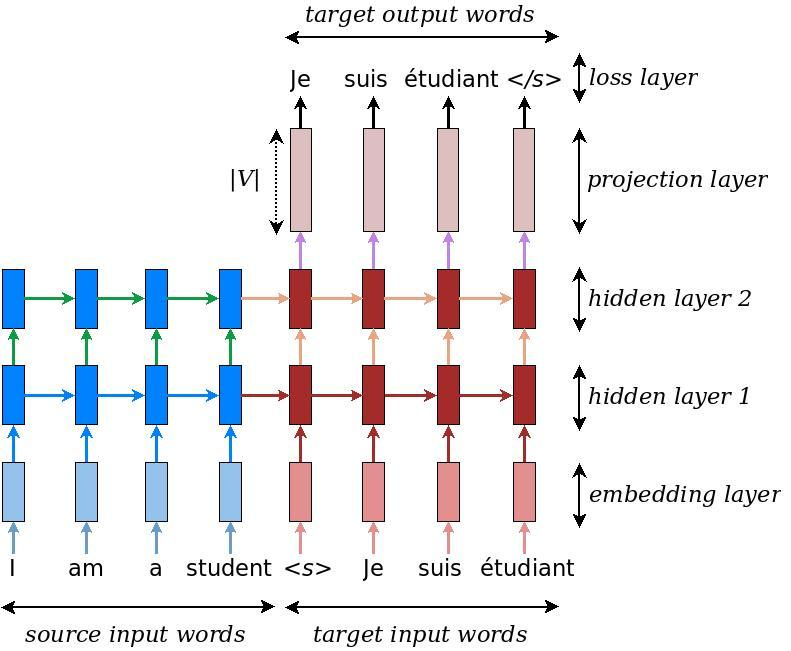
\includegraphics[width=0.75\textwidth]{seq2seq.jpg}
    \caption{Sequence to Sequence Model (Luong, 2017)}
  \end{center}
\end{figure}

\begin{figure}[H]
  \begin{center}
    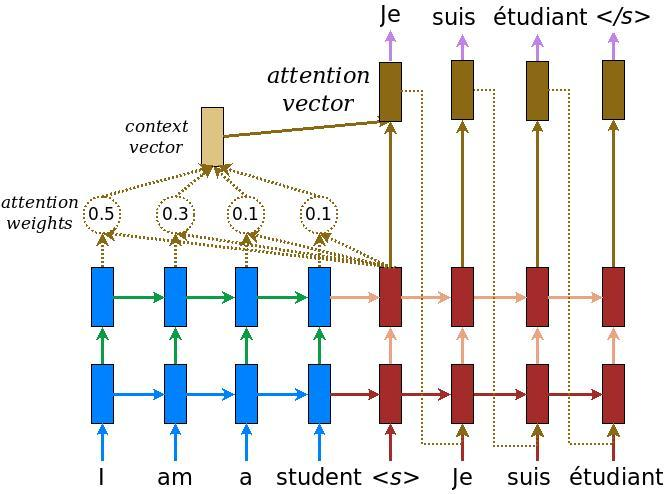
\includegraphics[width=0.75\textwidth] {attention_mechanism.jpg}
    \caption{Sequence to Sequence Model with Attention Mechanism (Luong, 2017)}
  \end{center}
\end{figure}

\clearpage

\section{Methodology}

  In this project there are two networks. A Convolutional Neural Network is used as a language classifier, to detect whether a given input is English or French. Next, a tensor2tensor network, specifically using Google's Transformer model, translates the given input to the opposite language. For example a given input is identified as English and translated to French. And vice versa.
  
  The convolutional network benefits in accuracy from specific characteristics of the input languages. For example, languages with special characters can be quickly identified. French has accented characters which are concatenated to English characters to form an alphabet of expected characters. This allows the CNN to easily identify input characters that will only appear in a certain language.

\begin{figure}[H]
  \begin{center}
    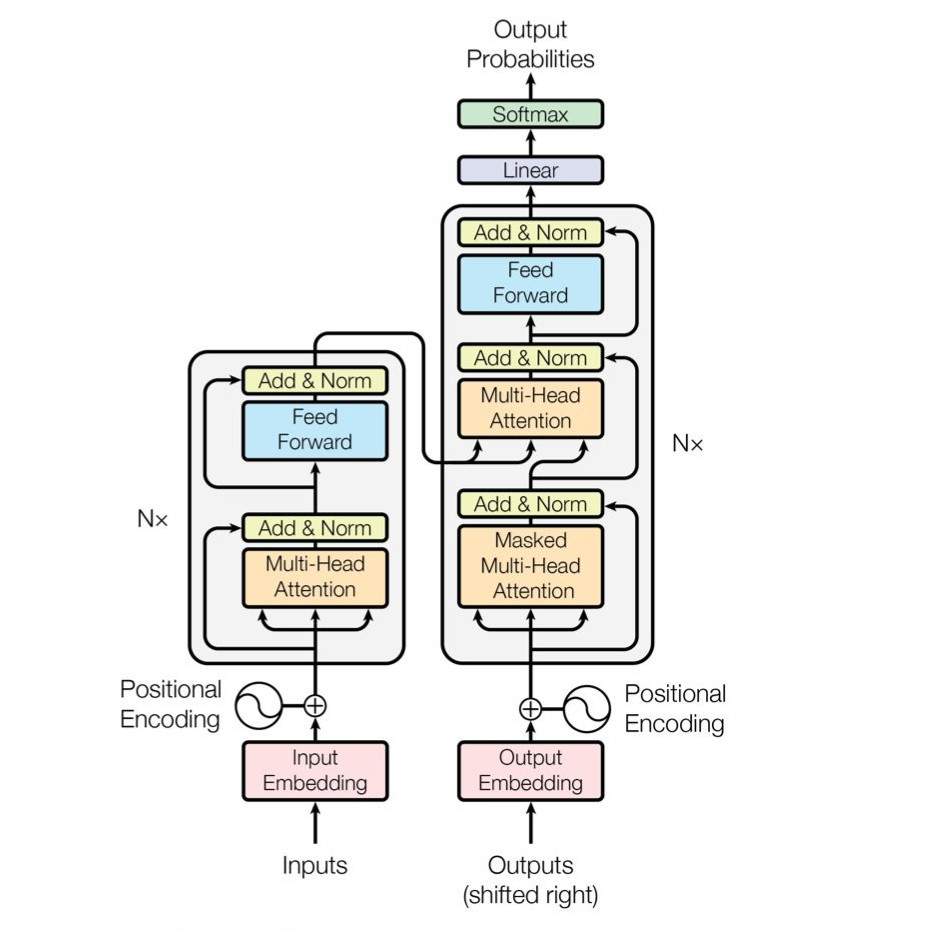
\includegraphics[width=0.8\textwidth] {transformer.jpg}
    \caption{Transformer Model architecture}
  \end{center}
\end{figure}

\clearpage

\section{Experiments}

  Datasets in Spanish were difficult to find, but there are many datasets in other languages. For training, the classifier and translation models were trained with WMT-small8k data set in English and French. In order to train translation, the model needs to study the target language and human corrected translations. It is not necessary to train the model with the input language and human corrected translations of the target language, but rather any human corrected language. In this way a trained model can train on multiple languages without need for datasets to overlap languages, this enables us to add a new language at a later date.

  The dataset is WMT's English-French small 8k vocab. This enabled both the translator and classifier to train using the same dataset. The small vocab size was necessary to train in time for submission.

\section{Discussion}
	The classifier's Keras Sequential model was able to reach near perfect validation accuracy in the first epoch. The test accuracy after 5 epochs was .
	The translation net takes significantly longer to train. After 2 days the validation esimated BLEU score was over 40. At the time of writing the estimated validation BLEU score is 49.1688.

\begin{figure}[H]
  \begin{center}
    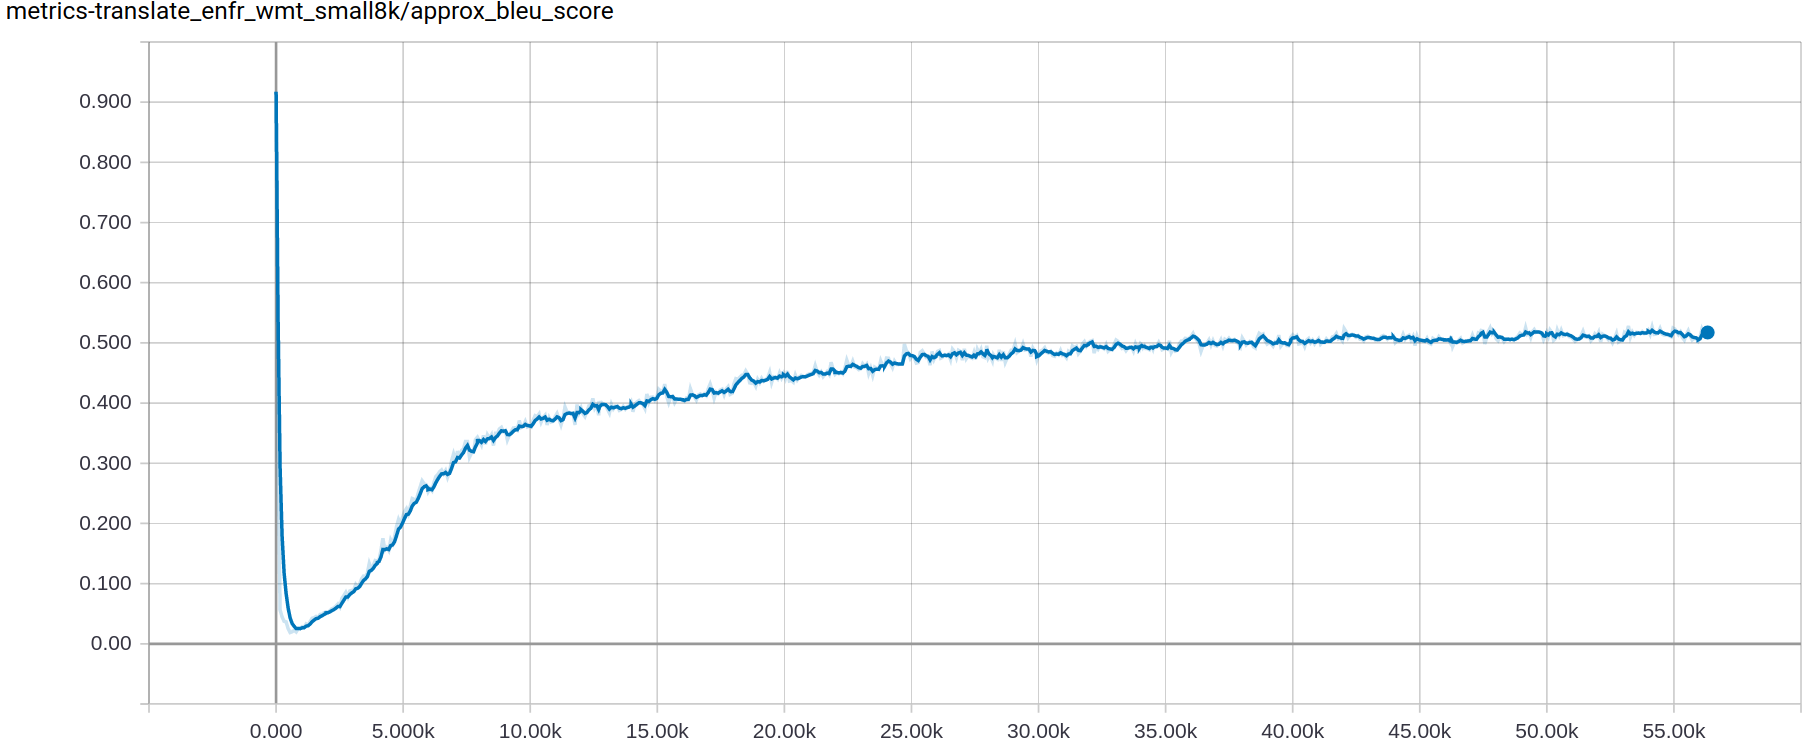
\includegraphics[width=0.8\textwidth] {BLEU.png}
    \caption{BLEU score after ~3 days}
  \end{center}
\end{figure}

\begin{figure}[H]
  \begin{center}
    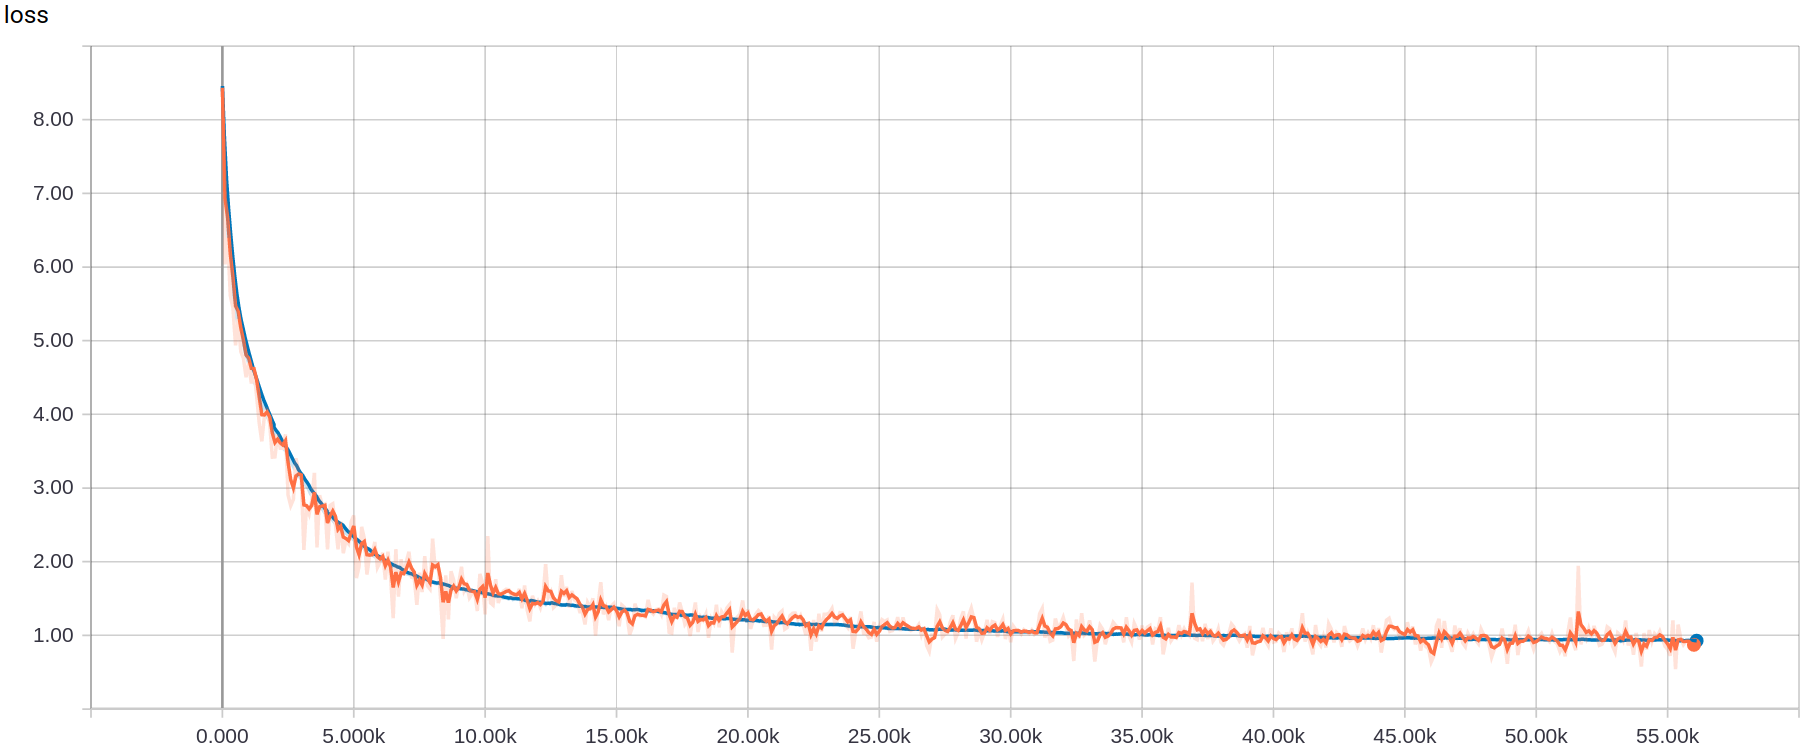
\includegraphics[width=0.8\textwidth] {loss.png}
    \caption{Loss after ~3 days}
  \end{center}
\end{figure}

\begin{figure}[H]
  \begin{center}
    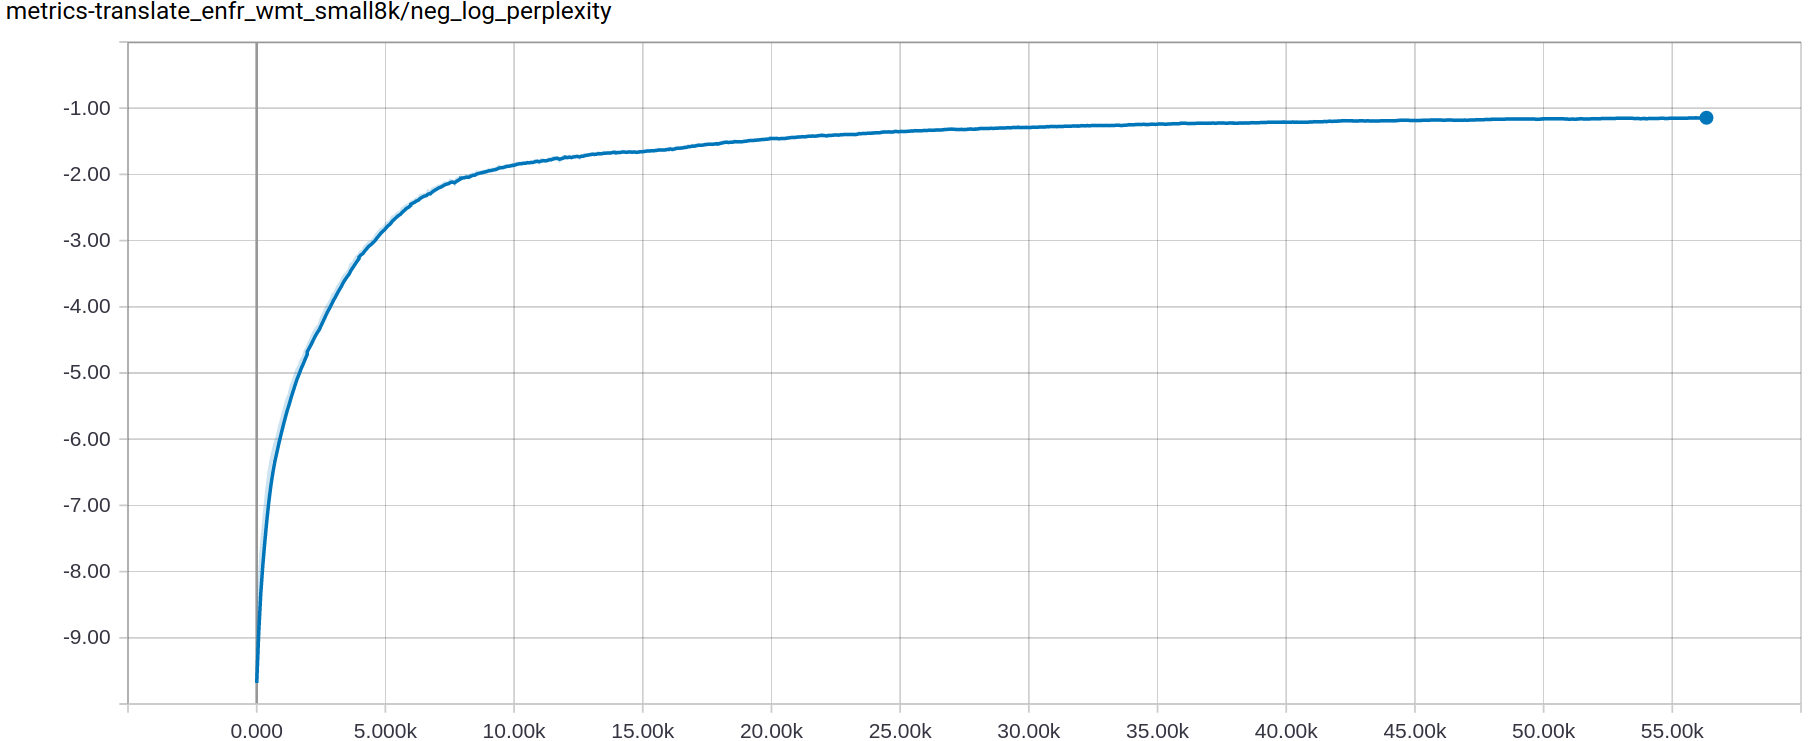
\includegraphics[width=0.8\textwidth] {neg_log_perp.png}
    \caption{Negative Log Perplexity after ~3 days}
  \end{center}
\end{figure}

\section{Conclusion}


\clearpage


\section{References}

\subsection{Further Reading}

https://github.com/tensorflow/nmt

https://github.com/google/seq2seq

https://github.com/tensorflow/tensor2tensor

http://www.nltk.org/

https://nlp.stanford.edu/projects/nmt/

https://research.googleblog.com/2017/07/building-your-own-neural-machine.html

https://sites.google.com/site/acl16nmt/

https://github.com/lmthang/thesis

https://google.github.io/seq2seq/data/

http://www.statmt.org/europarl/

https://conferences.unite.un.org/UNCorpus

http://www.statmt.org/wmt17/translation-task.html

\subsection{Sources}

Johnson, Melvin, et al. "Google’s Multilingual Neural Machine Translation System: Enabling Zero-Shot Translation." Arxiv. 2016.

(https://arxiv.org/pdf/1611.04558v1.pdf)
\newline

Sutskever, Ilya, et al. "Sequence to Sequence Learning with Neural Networks." NIPS. 2015.

(https://papers.nips.cc/paper/5346-sequence-to-sequence-learning-with-neural-networks.pdf)
\newline

Cho, Kyunghyun, et al. "Learning Phrase Representations using RNN Encoder–Decoder for Statistical Machine Translation." ACLweb. 2014.

(http://aclweb.org/anthology/D/D14/D14-1179.pdf)
\newline

Bahdanau, Dzmitry, et al. "Neural Machine Translation By Jointly Learning To Align and Translate." Arxiv. 2016.

(https://arxiv.org/pdf/1409.0473.pdf)
\newline

Luong, Minh-Thang, et al. "Effective Approaches to Attention-based Neural Machine Translation." Arxiv. 2015.

(https://arxiv.org/pdf/1508.04025.pdf)
\newline

Wu, Yonghui, et al. "Google’s Neural Machine Translation System: Bridging the Gap between Human and Machine Translation." Arvix. 2016.

(https://arxiv.org/abs/1609.08144)
\newline

Neubig, Graham, et al. "Neural Machine Translation and Sequence-to-sequence Models: A Tutorial." Arvix. 2017.

(https://arxiv.org/abs/1703.01619)
\newline

\end{document}
